\documentclass[11pt, preprint]{aastex}
\usepackage{xcolor}
\usepackage{hyperref}
\usepackage{rotating}  

\usepackage{environ}
\usepackage{amsmath}

\newcommand{\todo}[1]{{\bf #1}}
\newcommand{\Sersic}{S\'ersic}      
\newcommand{\dd}[1]{\ensuremath{{\rm d}#1}}
\newcommand{\mat}[1]{\ensuremath{{\bf #1}}}

\newif\ifanswers

\NewEnviron{answer}[1][]{\ifanswers\color{blue}\expandafter\BODY
{\par \it #1}\fi}

\DeclareMathOperator\erf{erf}

\newenvironment{ditemize}
{ \begin{list}{}{%
\setlength{\topsep}{0pt}% 
\setlength{\partopsep}{3pt}% 
\setlength{\itemsep}{1pt}\setlength{\parsep}{1pt}% 
\setlength{\itemindent}{0pt}\setlength{\listparindent}{12pt}%
\setlength{\leftmargin}{24pt}\setlength{\rightmargin}{0in}%
\setlength{\labelsep}{6pt}\setlength{\labelwidth}{6pt}%
\renewcommand{\makelabel}{\makebox[\labelwidth][l]{$\bullet$\hspace{\fill}}}}}
{\end{list}}


\answersfalse

\begin{document}

\title{\bf Miscellaneous Notes}

\section{Ultra diffuse galaxies (UDGs)}

Generally defined as galaxies with central surface brightness fainter
than 24 mag arcsec$^{-2}$. These have been found by the DragonFly
collaboration, by HyperSuprimeCam, and are expected in Rubin
Observatory and Roman Space Telescope data. Some of them at least are
highly dark matter dominated, based on measured velocity dispersion
but also on their number of globular clusters (i.e. $10^{12}$
$M_\odot$ halo; Wasserman et al. 2019).

They can have very dense nuclear star clusters, which can hold around
1\% of the stars (SMUDGES studies from Zaritzky et al, Khim et al).

\section{Simulation of Spiral Galaxy Formation}

\section{Molecular cloud properties vs. galaxy and subgalaxy
  environment}

There are a number of detailed (10-100 pc resolution) CO maps of
nearby galaxies from several recent investigations
(\citealt{schinnerer13a, donovan-meyer13a, leroy21a, koda23a}). As
reviewed in the introduction to \citet{finn23a}, these observation
find that spiral arms have molecular gas which is higher surface
density than in the interarm regions, with a shallower slope for the
cloud mass distribution, and a higher truncation mass. This coincides
with higher star formation rates, such that the depletion time is
similar (\citealt{querejeta21a}).

\citet{finn23a} examine a barred spiral (NGC 1313) and a flocculent
spiral (NGC 7793), which have similar masses and total star formation
rates. NGC 7793 does have massive clouds, but they have lower
pressures and densities and are less likely to form stars.

\section{AGN in Dwarf Galaxies}

Since around 2010 there have been an increasing number of detections
of AGN in dwarf galaxies.  Reines et al. (2013) searched the NASA
Sloan Atlas using the optical BPT diagram and found a fraction around
0.13\% for galaxies with $M<3\times 10^9 M_\odot$, which is
considerably smaller than the fraction for higher mass galaxies.
Trump et al. (2015) looked at the selection effects in detecting AGN
through BPT, and in that paper the lower AGN fraction at lower masses
could be mostly explained with a constant Eddington ratio
distribution. Satyapal et al (2014) and Marleau et al (2014) have both
searched for dwarf galaxy AGN in the mid-IR, finding larger
fractions. Sartori et al. (2015) repeated both analyses in the optical
and in the mid-IR. However, the mid-IR studies have not accounted for
selection effects.

Penny et al. (2018) found several quenched galaxies with AGN and
apparent outflow signatures (only one with mid-IR signatures of an
AGN); these may be similar to higher-mass ``red geyser'' galaxies.
Manzano-King et al. (2019) used Keck/LRIS and Liu et al (2020) used
Keck/KCWI 

\section{AGN Radio Loud, Radio Quiet Dichotomy}

It is believed that AGN have a bimodal dichotomy between radio loud
and radio quiet populations.  Strittmatter et al (1980) pointed this
out, and his results appeared to be confirmed by Kellerman et al
(1989). It is from Kellerman that we get the standard definition of
radio loudness, which is $R = f_{\nu,galax {\rm 6~cm}} / f_{\nu,
  4400\AA}$. The evidence for the radio loudness bimodality from that
paper can be found in Figure \ref{fig:kellerman89a}.

Papers to look at:
 * Ivezic (2002), Laor (2003), Ho (2002)

\begin{figure}
  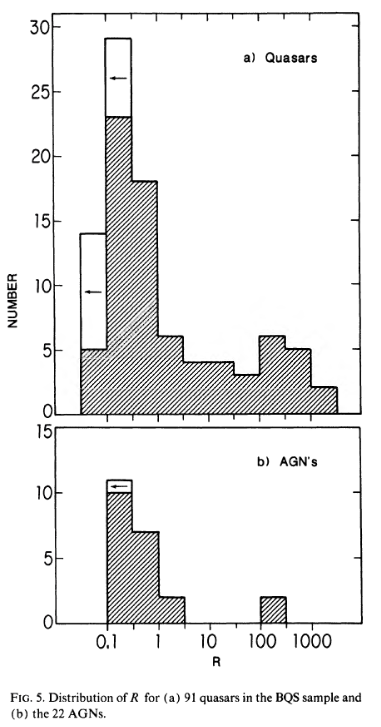
\includegraphics{kellerman89a.png}
  \caption{\label{fig:kellerman89a} From Kellerman et al (1989).}
\end{figure}

\section{Gas stripping and pressure}

Stephanie Tonneson talks about the effect of ram pressure stripping on
SFR and molecular gas formation in galaxies. Claim is that Moretti
2020 shows this happening. Also Peluso et al (using MaNGA) claims high
AGN fraction for RPS galaxies; this is a comparison between MaNGA and
a bespoke sample of RPS galaxies from MUSE samples (GASP) and the
literature. The definiti on of AGN-ness uses the number of Seyfert or
LINER like spaxels within 3 arcsec; also from the {\it parent} sample
they exclude all galaxies without the necessary lines for BPT. Looking
at this in simulations (Akerman, Tonneson, et al), and testing subgrid
models with this.

\section{Prolate galaxies at high redshift}

Pandya claims that 50--80\% of galaxies at $z\sim2$---8 are {\it
  prolate}, based on the projected $b/a$ distribution. He has tested
the surface brightness completeness which does not seem like a
problem. The inference he is doing accounts for both the size and the
$b/a$. He has proposed NIRSpec spectra to get emission line dynamics
at least; prolate things should not have a rotation curve like a
disk. He thinks these shapes are driven by the cosmic web filaments;
this is testable via intrinsic alignment tests.

\section{Compact and Extended Galaxy AGN population}

Aird, Coil, Kocevski (2022) claim AGN enhancement for compact star
forming galaxies, based on X-ray and CANDELS.

\end{document}

 


 
